% !TEX encoding = UTF-8 Unicode
\documentclass[a4paper]{article}

\usepackage{color}
\usepackage{url}
\usepackage[T2A]{fontenc}
\usepackage[utf8]{inputenc}
\usepackage{graphicx}

\usepackage[english,serbian]{babel}

\usepackage[unicode]{hyperref}
\hypersetup{colorlinks,citecolor=green,filecolor=green,linkcolor=blue,urlcolor=blue}

\usepackage{listings}

\newtheorem{primer}{Primer}[section]

\definecolor{mygreen}{rgb}{0,0.6,0}
\definecolor{mygray}{rgb}{0.5,0.5,0.5}
\definecolor{mymauve}{rgb}{0.58,0,0.82}

\lstset{ 
  backgroundcolor=\color{white},
  basicstyle=\scriptsize\ttfamily,
  breakatwhitespace=false,
  breaklines=true,
  captionpos=b,
  commentstyle=\color{mygreen},
  deletekeywords={...},            
  escapeinside={\%*}{*)},          
  extendedchars=true,
  firstnumber=1000,              
  frame=single,	                
  keepspaces=true,
  keywordstyle=\color{blue},     
  language=Python,                
  morekeywords={*,...},
  numbers=left, 
  numbersep=5pt,                  
  numberstyle=\tiny\color{mygray}, 
  rulecolor=\color{black},
  showspaces=false,
  showstringspaces=false,
  showtabs=false,
  stepnumber=2, 
  stringstyle=\color{mymauve},
  tabsize=2,
  title=\lstname
}

\begin{document}

\title{Programski jezik F\#\\ \small{Seminarski rad u okviru kursa\\Metodologija stručnog i naučnog rada\\ Matematički fakultet}}

\author{Tijana Todorov, Tamara Garibovic,\\ David Nedeljkovic, Mihajlo Vicentijevic \\ tijana.todorov710@gmail.com, t.garibovic1995@gmail.com, \\ dnedeljkovic710@gmail.com, mihajlovicent@gmail.com}

%\date{9.~april 2015.}

\maketitle

\abstract{
Dodati na kraju sazetak.}

\tableofcontents

\newpage

\section{Uvod}
\label{sec:uvod}

Dodati na kraju uvod u temu i obavezno izmeniti trenutni radni naslov.

\section{U 2018. godini F$\#$ opisan je u dokumentaciji kao "funkcionalni programski jezik koji se pokrece na .NET platformi" \cite{early_history},ali odakle je on potekao?}
\label{sec:poreklo}

Istorija programskog jezika F$\#$ datira jos od 1970. godine pa sve do danas. U ranim 70-im godinama na Univerzitetu u Edinburgu Robin Milner sa jos nekoliko svojih kolega razvija jezik ML (Meta-Language) baziran na programskom jeziku LISP. Njegova onsnovna namena bila je pragmaticnog karaktera. Osmisljen je da pomogne u dokazivanju LCF (Logical computable functions) \cite{Milner:1972:LCF:891954} teorema. ML jezik je koren svih jezika koji pripadaju familiji strogo tipiziranih funkcionalnih jezika, kao npr: Miranda, Haskell, Standard ML, Ocaml, EdinburghML, ReasonML, PureScript, a medju njima i F$\#$.

Sve do danas kljucne ideje ove familije jezika ostaju osnova jezika F$\#$ koji se nadogradjivao kasnije iz dana u dan. 

Tokom 80-ih godina dolazi do velike ekspanzije u kompjuterskoj industriji. Kako su se brzo razvijali softverski alati tako su se takodje pojavljivali novi jezici i programske paradigme. U tom periodu i Microsoft dozivljava veliku ekspanziju kao kompanija koja razvija operativne sisteme i aplikacije. Medjutim, u ovom periodu, a najvise u kasnim 80-im godinama pojavljuje se novi, objektno-orjentisani talas razmisljanja u programiranju koji veoma utice na razvoj softvera.

Pocetkom 90-ih godina dok je Microsoft tezio da odrzi monopol na trzistu i dok je u fokusu i dalje bila objektno-orjentisana paradigma, strogo tipizirani funkcionalni jezici bili su manje aktivni i okrenuti su ka razvitku na drugim poljima. Njihova primena uglavnom je imala ulogu u pronalazenju bagova, odrzavanju sistema i verifikaciji hardvera i softvera. Primeri jezika koji su se koristili za izgradnju oviakvih sistema su: Edinburgh ML, Standard ML, Ocaml, Caml Light, LISP. Takodje su neki funkcionalni jezci razvijeni u cilju istrazivanja u okviru paralelnog programiranja, kao sto su Parallel ML i vrsta paralelnog Haskell-a \cite{early_history}. 

\subsection{Zasto je nastao jezik F$\#$?}
\label{subsec:nastanak}

Tokom 90-ih godina Microsoft razvija .NET \cite{microsoft_.net,early_history} platformu za razvoj softvera. Ideja je bila da se omoguci medjusobna kompatibilnost vise programskih jezika, odnosno da svaki jezik podrzan na ovoj platformi moze koristiti kôd nekog drugog jezika platforme. Glavni cilj Microsoft-a bio je da se na ovoj platformi podrzi sto veci broj jezika iz razlicitih paradigmi. 

U okviru ovoga Don Sym razija projekat SML.NET koji je za ideju imao preusmeravanje Standard ML-a na .NET. Sistem je imao visok kvalitet, ali nije bio usvojen od strane programera. Pocetkom 2000-ih platforma .NET je vec uveliko zazivela, ali za jezik SML.NET nije bilo veceg interesovanja. Autor je imao veliku zelju da implementira strogo tipiziran funkcionalni jezik na nacin koji bi zainteresovao veliki broj programera. U razmatranje ulazi i jezik OCaml, ali prethodno dolazi do pokusaja implementacije Haskell-a za .NET. Ovaj pokusaj bio je samo delimicno uspesan i primenjen na malim programima. Rad na daljoj implementaciji je zaustavljen.

U decembru 2001. godine Don Syme u razmatranje vraca jezik OCaml u cilju da se implementira za .NET platformu i razvija projekat Caml.NET koji ce se kasnije preimenovati u F$\#$.

Inicijalna ideja F$\#$ programskog jezika bila je jednostavna. Trebalo je da poveze prednosti OCaml programskog jezika sa prednostima .NET platforme. 2002. godine pojavljuje se prva verzija F$\#$ 0.5 koja bila je slabo primecena. Don Syme 2004. godine nastavlja intenzivno da razvija ovaj jezik, a pocetkom 2005. godine izbaciuje prvu potpunu verziju ovog programskog jezika \cite{early_history}.
Poslednja aktuelna verzija ovog jezika je F$\#$ 4.1 \cite{fsharp}.

\subsection{Koji programski jezici su najvise uticali na razvoj jezika F$\#$?}
\label{subsec:uticaj}

Najveci znacaj za razvoj jezika F$\#$ imaju jezici SML (Standard ML) i CAML (Categorical Abstarct Machine Language) porodica jezika koja je razvijana na Nacionalnom institutu za istrazivanje informatike i automatizacije u Francuskoj 1994.godine \cite{Harrop:2008:FS:1481410}. U okviru ovog projekta pod nazivom “Cristal project” razvija se jezik Objective Caml koji ima veoma visoke performanse i naucnici ga koriste na Linux i MAC OS X platformama. Kao sto je vec ranije opisano, ovaj jezik i .NET platforma imali su najveci uticaj na razvoj jezika F$\#$. Na slici \ref{fig:stablo} moze se videti deo razvojnog stabla koji ovo prikazuje.

\begin{figure}[h!]
\begin{center}
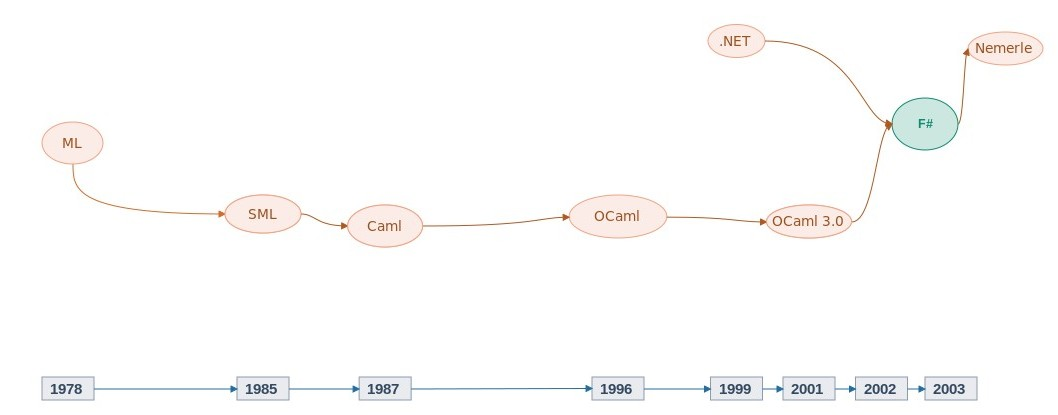
\includegraphics[scale=0.29]{stablo.jpg}
\end{center}
\caption{Razvojno stablo}
\label{fig:stablo}
\end{figure}


\section{Primena i mogucnosti}
\label{sec:primena}

Snaga F$\#$ programskog jezika lezi u svedenoj sintaksi koja omogućava laku čitljivost kôda, kao i efikasan razvoj programa koji zahtevaju primenu složenih matematičkih algoritama. Jezik omogućava brzo generisanje prototipova i njihovu brzu transformaciju u produkcioni kôd. Kôd napisan u F$\#$-u lako se može paralelizovati, što je posebno značajno danas kada svi novi računari imaju više jezgara. F$\#$ danas ima siroku primenu u obradi baza podataka, finansijskog modelovanja, statistici i bioinformatici. Takodje domen primene iz dana u dan raste.

F$\#$ je jezik koji ima pretezno funkcionalne karakteristike, ali on je svoju primenu pronasao u jos mnogo vrsta programiranja. Neki od njih su: imperativno, objektno-orjentisano, paralelno, distribuirano, asinhrono, meta programiranje, veb programiranje, skript programiranje, analiticko programiranje, i sl. Danas se on moze koristiti na velikom broju sistema, kao sto su: Linux, MAC, Windows, Android, iOS, i sl. O tome ce biti vise reci u nastavku. 

\section{Zaključak}
\label{sec:zakljucak}

Sta je zakljucak celog rada.

\addcontentsline{toc}{section}{Literatura}
\appendix
\bibliography{seminarski} 
\bibliographystyle{plain}

\appendix
\section{Dodatak}
Ovde pišem dodatne stvari, ukoliko za time ima potrebe.
Ovde pišem dodatne stvari, ukoliko za time ima potrebe.
Ovde pišem dodatne stvari, ukoliko za time ima potrebe.
Ovde pišem dodatne stvari, ukoliko za time ima potrebe.
Ovde pišem dodatne stvari, ukoliko za time ima potrebe.


\end{document}